\documentclass{article}
\usepackage[utf8]{inputenc}
\usepackage{graphicx}
\usepackage{amsmath}

\usepackage{psfrag}
\begin{document}

\pagestyle{empty}
\psfrag{\{EMPTY TITLE\}}{
	$ $
}
\psfrag{\{X LABEL\}}{
	\begin{picture}(0,0)
	\put(-95, -5){Liczba wierzchołków w grafie $G$ ($\left| E \right| = \frac{1}{10} \cdot \binom{\left| V \right|}{2}$)}
	\end{picture}
}
\psfrag{\{Y LABEL\}}{
	\begin{picture}(0,0)
	\put(-30, 10){Czas działania $ \left[ ms \right] $}
	\end{picture}
}

\psfrag{INCREMENTALIMST1XXXXXXXXXXXXXXXXXXXXXXXXXXXXX}{$\textsc{incremental-mst} \left( G, T^{\ast}_{\textbf{s}}, \textbf{s}^{\prime}, k, L, U \right)$}
\psfrag{INCREMENTALIMST2XXXXXXXXXXXXXXXXXXXXXXXXXXXXX}{$\textsc{incremental-mst}^{\prime} \left( G^{\ast}, T^{\ast}_{\textbf{s}}, \textbf{s}^{\prime}, k, L, U \right)$}
\psfrag{LINEARMODELXXXXXXXXXXXXXXXXXX}{\scriptsize model programowania liniowego $4.14$}

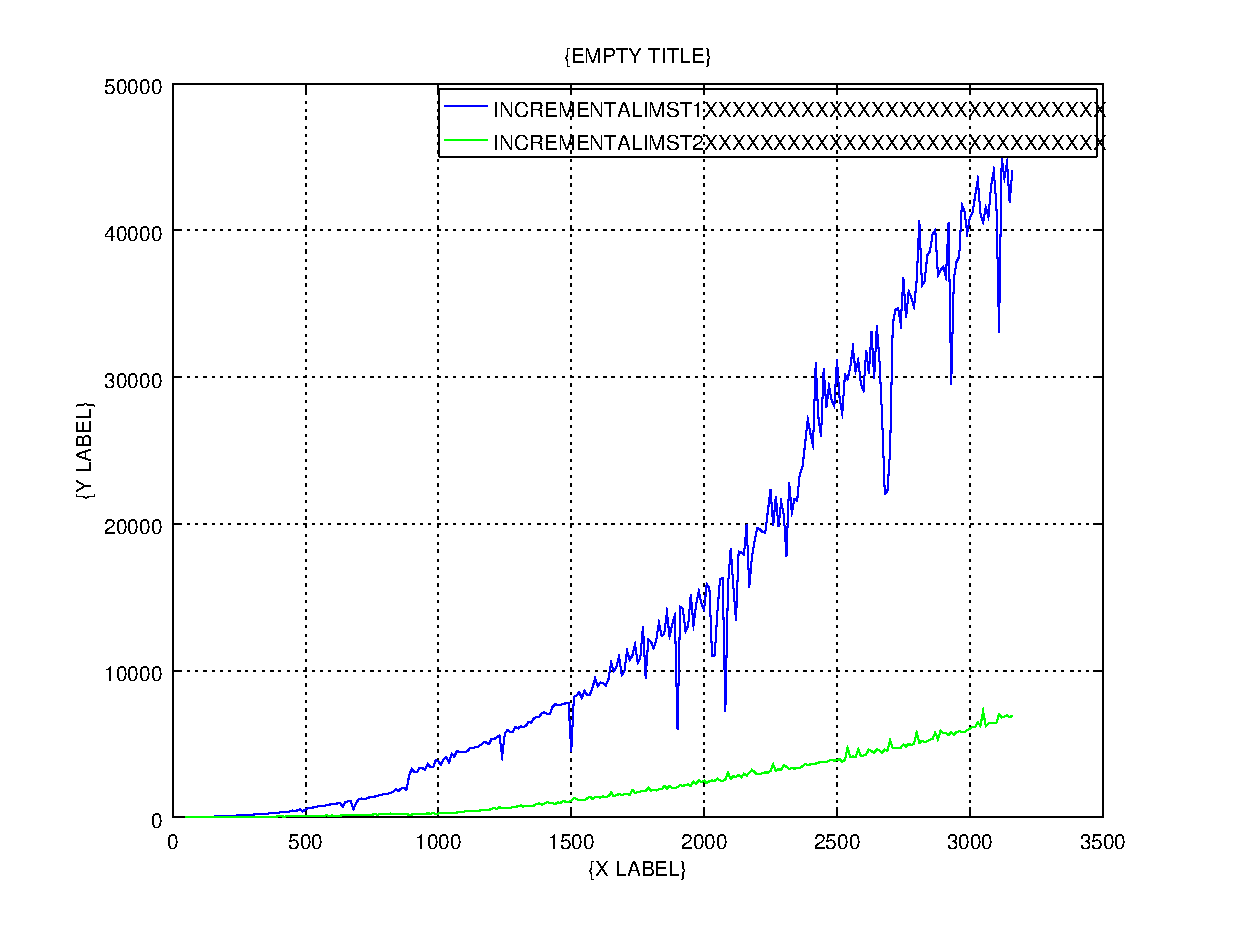
\includegraphics[width=\textwidth]{out}
\end{document}